
% last updated in April 2002 by Antje Endemann
% Based on CVPR 07 and LNCS, with modifications by DAF, AZ and elle, 2008 and AA, 2010, and CC, 2011; TT, 2014; AAS, 2016

\documentclass[runningheads]{llncs}
\usepackage{graphicx}
\usepackage{amsmath,amssymb} % define this before the line numbering.
\usepackage{ruler}
\usepackage{color}
\usepackage[width=122mm,left=12mm,paperwidth=146mm,height=193mm,top=12mm,paperheight=217mm]{geometry}

\graphicspath{{../pdf/}{..\DD2424-Project\plots}}

\begin{document}
% \renewcommand\thelinenumber{\color[rgb]{0.2,0.5,0.8}\normalfont\sffamily\scriptsize\arabic{linenumber}\color[rgb]{0,0,0}}
% \renewcommand\makeLineNumber {\hss\thelinenumber\ \hspace{6mm} \rlap{\hskip\textwidth\ \hspace{6.5mm}\thelinenumber}}
% \linenumbers
\pagestyle{headings}
\mainmatter
\def\ECCV16SubNumber{***}
\title{DD2424 Project - Character-Level Text Classification with different RNN Architectures}
\\Authors\\
Ching-an Wu 
Rithika Harish Kumar 
Mathilda Strandberg von Schantz

\maketitle

%The final report should include the following sections:

\begin{abstract}
% • Abstract: Where you give an overview of the task and the findings
% of your work in a nutshell.

A character-level RNN is used to classify text(words) to the respective categories using Pytorch. This is an extension of a tutorial\cite{maintutorial}. But the tutorial has implemented only Recurrent neural networks. Where as we have also implemented Long short term memory and Gated recurrent unit. Also we have used a different dataset.   

\dots
\keywords{We would like to encourage you to list your keywords within
the abstract section}
Character-Level, Text classification, RNN, LSTM, GRU, Pytorch 
\end{abstract}


\section{Introduction}

% • Introduction/Problem formulation: Motivate the problem you
% are trying to solve, attempt to make an intuitive description of the
% problem and also formally define the problem. (1-2 pages including
% title, authors and abstract)

We are looking at a text classification problem with short text and character-level classification. The texts we are looking at are names of cities, and the classes are the names of the country the city belongs to. There are circa 240 categories (countries) in the data set, but we will limit the number of categories so as not to make the categories too unevenly distributed (ie remove countries with too few cities in the data set).

We will be using character-level classification. This means that the network processes the input one character at a time. Each character results in an output consisting of the probabilities for each letter for the next character. If we have a 58-character alphabet, the hidden state will consist of the probability of each of those 58 characters for the next letter in the sequence. So for each character, one such prediction is produced, as well as a hidden state, which is fed into the next step.

Short-text classification is hard in that there is less information to go off with little to no grammar or syntax. Some applications of short-text classification include search queries and information retrieval, mapping a product name to its associated product, the classification of titles, questions, sentences, and short messages.

The inspiration for the project is a tutorial in which a recurrent network is used to classify names as belonging to certain nationalities. To start with, the model of that tutorial is to be replicated, then additional architectures will be implemented and compared. Questions we ask ourselves include: to what degree would a deeper network help in this problem? What sort of architectures are good in this application? Would an LSTM-layer in the recurrent network give better results? 

To measure the success of the text classification, we will look at the precision, recall and f1-score of each category in the data set. This because it gives a more nuancued evaluation than accuracy, seeing as how the data set used is heavily skewed. Furthermore, we will visualize the results with a confusion matrix.


\section{Background}

% • Background: summarize a few notable approaches/papers tackling
% the same problem. The selection should cover different possible tech-
% niques that can be (have been) used for the same task with success.
% Also, it is good to mention other recognition/synthesis tasks that use
% the same deep learning technique as yours. (1-2 pages)

\section{Theory}

This section consists of the working\cite{colah} of RNN, LSTM and GRU
 
\subsection{RNN - Recurrent Neural Networks}

Traditional neural networks do not use reasoning based on the previous events to inform the later ones. To allow information to persist, RNNs were used. These are networks with loops.

\begin{figure}[h!]
\centering
        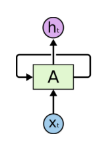
\includegraphics[width=0.5\linewidth]{plots/working_rnn.png}
    \caption{RNN Model}
\end{figure}

The above figure has a chunk of neural network A, with $x_t$ as input and $h_t$ as output. The loop allows information to be passed from one step to another. The basic equation is as follows:

\[state = W_x x_t + W_h h_{t-1} + b \]
\[h_t = tanh(state) \]

Although RNNs help in keeping the information, it is difficult to have long term dependencies. In practise, RNNs dont seem to learn it. So, LSTM came into play.

\subsection{LSTM - Long short term memory}

LSTM is a special kind of RNN which is capable of long-term dependencies. It is done by having a cell state. Cell states are regulated by three gates called forget($f_t$), input($i_t$) and output($o_t$). They help in optionally letting information. Gates are composed of sigmoid neural net layer and pointwise multiplication operation.

\begin{figure}[h!]
\centering
        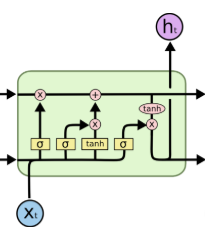
\includegraphics[width=0.5\linewidth]{plots/working_lstm.png}
    \caption{RNN}
\end{figure}

First step is to decide what information to throw away from cell state.

\[f_t = \sigma(W_f.[h_{t-1},x_t] + b_f) \]

Second step is to create a update. So decide what information to be stored in cell state. Next, a tanh layer creates a vector of candidate values($~C_t$) to be added.

\[i_t = \sigma(W_i.[h_{t-1},x_t] + b_i) \]
\[~C_t = tanh(W_c.[h_{t-1},x_t] + b_c) \]
\[C_t = f_t * C_{t-1} + i_t * ~C_t \]

Finally, we decide what parts of the cell to output by sigmoid layer. Then run a tanh and multiply with the output of sigmoid layer.

\[o_t = \sigma(W_o.[h_{t-1},x_t] + b_o) \]
\[ h_t = o_t * tanh(C_t)\]

This way LSTM has the ability to allow which information to pass through.
 
\subsection{GRU -  Gated Recurrent Unit}

The idea behind a GRU layer is quite similar to that of a LSTM layer except that GRU has only two gates. The input and forget gates are coupled by an update gate ($z_t$) and the reset gate ($r_t$) is applied directly to the previous hidden state.  

\begin{figure}[h!]
\centering
        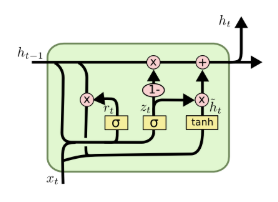
\includegraphics[width=0.5\linewidth]{plots/working_gru.png}
    \caption{RNN}
\end{figure}

\[z_t = \sigma(W_z.[h_{t-1},x_t]) \]
\[r_t = \sigma(W_r.[h_{t-1},x_t]) \]
\[~h_t = tanh(W.[r_t * h_{t-1},x_t]) \]
\[h_t = (1-z_t) * h_{t-1} + z_t * ~h_t \]

Intuitively, the reset gate determines how to combine the new input with the previous memory, and the update gate defines how much of the previous memory to keep around. If we set the reset to all 1’s and  update gate to all 0’s we again arrive at our plain RNN model.

\section{Approach}
% • Approach: Describe the final approach you are take for this problem.
% For instance, here you would describe the details of the network’s
% architecture. What training parameters and techniques you have used.
% The computational complexity of your model. And similar questions.
% To help explain your approach please make figures to accompany your
% text description. (1-3 pages)

\section{Experiments}


\section{Results}
\section{Conclusions}

% • Experiments/Results/Conclusions: In this section, you should
% present the results you achieved with various experiments. The re-
% sults can be presented in tables, plots, etc. Explain what conclusions
% you can draw from these set of experiments? The set of experiments
% and results reported here should justify some of the design choices
% described in the previous sections. (3-6 pages)

As \cite{Alpher04} said.

% • References: It is extremely important to make sure all the content
% from other sources and the ideas that you build on are properly cited.


% Both positive and negative results should be reported. A discussion re-
% garding why certain techniques worked better than the others is necessary.
% Students are also encouraged to take initiatives in trying out new techniques,
% beyond those discussed at the lectures.
% The stated number of pages above is a guideline, one can go beyond that or
% slightly below. The whole report should be between 7-14 pages.


\bibliographystyle{splncs}
\bibliography{egbib}
\begin{thebibliography}

\bibitem{maintutorial}
\\\texttt{https://github.com/spro/practical-pytorch/blob/master/char-rnn-classification/char-rnn-classification.ipynb}

\bibitem{colah}
\\\texttt{https://colah.github.io/posts/2015-08-Understanding-LSTMs/}

\end{thebibliography}
\end{document}
